\section{Технический проект}
\subsection{Общая характеристика организации решения задачи}

Необходимо спроектировать и разработать приложение, который должен способствовать популяризации ролевых игр.

Приложение представляет собой набор взаимосвязанных различных окон, которые сгруппированы по разделам, содержащие текстовую, графическую информацию. Приложение располагается на компьютере.

\subsection{Обоснование выбора технологии проектирования}

На сегодняшний день информационный рынок, поставляющий программные решения в выбранной сфере, предлагает множество продуктов, позволяющих достигнуть поставленной цели – разработки приложения.

\subsubsection{Описание используемых технологий и языков программирования}

В процессе разработки приложения используются программные средства и языки программирования. Каждое программное средство и каждый язык программирования применяется для круга задач, при решении которых они необходимы.

\subsubsection{Язык программирования Python}

Python –  высокоуровневый язык программирования общего назначения с динамической строгой типизацией и автоматическим управлением памятью, ориентированный на повышение производительности разработчика, читаемости кода и его качества, а также на обеспечение переносимости написанных на нём программ. Язык является полностью объектно-ориентированным в том плане, что всё является объектами. Необычной особенностью языка является выделение блоков кода отступами. Синтаксис ядра языка минималистичен, за счёт чего на практике редко возникает необходимость обращаться к документации. Сам же язык известен как интерпретируемый и используется в том числе для написания скриптов. Недостатками языка являются зачастую более низкая скорость работы и более высокое потребление памяти написанных на нём программ по сравнению с аналогичным кодом, написанным на компилируемых языках, таких как C или C++.

Python — это язык программирования, который широко используется в интернет-приложениях, разработке программного обеспечения, науке о данных и машинном обучении (ML). Разработчики используют Python, потому что он эффективен, прост в изучении и работает на разных платформах. Программы на языке Python можно скачать бесплатно, они совместимы со всеми типами систем и повышают скорость разработки.

\paragraph{В чем заключаются преимущества языка Python?}
Язык Python имеет следующие преимущества:

Разработчики могут легко читать и понимать программы на Python, поскольку язык имеет базовый синтаксис, похожий на синтаксис английского. 
Python помогает разработчикам быть более продуктивными, поскольку они могут писать программы на Python, используя меньше строк кода, чем в других языках.
Python имеет большую стандартную библиотеку, содержащую многократно используемые коды практически для любой задачи. В результате разработчикам не требуется писать код с нуля.
Разработчики могут легко сочетать Python с другими популярными языками программирования: Java, C и C++.
Активное сообщество Python состоит из миллионов поддерживающих разработчиков со всего мира. При возникновении проблем сообщество поможет в их решении.
Кроме того, в Интернете доступно множество полезных ресурсов для изучения Python. Например, вы можете легко найти видеоролики, учебные пособия, документацию и руководства для разработчиков.
Python можно переносить на различные операционные системы: Windows, macOS, Linux и Unix.
\paragraph{Где применяется Python?}
Язык Python имеет несколько стандартных примеров использования при разработке приложений, в числе которых:

Веб-разработка на стороне сервера
Веб-разработка на стороне сервера включает в себя сложные серверные функции, с помощью которых веб-сайты отображают информацию для пользователя. Например, веб-сайты должны взаимодействовать с базами данных и другими веб-сайтами, а также защищать данные при их отправке по сети. 

Python полезен при написании серверного кода, поскольку он предлагает множество библиотек, состоящих из предварительно написанного кода для сложных серверных функций. Также разработчики используют широкий спектр платформ Python, которые предоставляют все необходимые инструменты для более быстрого и простого создания интернет-приложений. Например, разработчики могут создать «скелет» интернет-приложения за считанные секунды, потому что им не нужно писать код с нуля. Затем его можно протестировать с помощью инструментов тестирования платформы независимо от внешних инструментов тестирования.

Автоматизация с помощью скриптов Python
Язык скриптов — это язык программирования, который автоматизирует задачи, обычно выполняемые людьми. Программисты широко используют скрипты Python для автоматизации многих повседневных задач, среди которых:

Одновременное переименование большого количества файлов
Преобразование файла в другой тип файла
Удаление повторяющихся слов в текстовом файле
Выполнение базовых математических операций
Отправка сообщений электронной почты
Загрузка контента
Выполнение базового анализа журналов
Поиск ошибок в нескольких файлах
\paragraph{Наука о данных и машинное обучение}
Наука о данных извлекает ценную информацию из данных, а машинное обучение (ML) позволяет компьютерам автоматически учиться на данных и делать точные прогнозы. Специалисты по работе с данными используют Python для решения следующих задач:

Исправление и удаление неверных данных (очистка данных) 
Извлечение и выбор различных характеристик данных
Разметка данных добавляет данным значимые имена
Поиск статистической информации в данных
Визуализация данных с помощью диаграмм и графиков: линейных диаграмм, столбчатых диаграмм, гистограмм и круговых диаграмм

Специалисты по работе с данными используют библиотеки Python ML для моделей машинного обучения и создания классификаторов, которые точно классифицируют данные. Классификаторы на основе Python используются в различных областях и применяются для выполнения таких задач, как классификация изображений, текста и сетевого трафика, распознавание речи и распознавание лиц. Специалисты по работе с данными также используют Python для глубокого обучения — передовой техники машинного обучения.
Разработка программного обеспечения
Разработчики программного обеспечения часто используют Python для различных задач разработки и программных приложений, среди которых:

Отслеживание ошибок в программном коде
Автоматическая сборка программного обеспечения
Управление программными проектами
Разработка прототипов программного обеспечения
Разработка настольных приложений с использованием библиотек графического пользовательского интерфейса (ГПИ)
Разработка игр: от простых текстовых игр до сложных видеоигр
Автоматизация тестирования программного обеспечения
Тестирование программного обеспечения — это процесс проверки соответствия фактических результатов программного обеспечения ожидаемым результатам, который позволяет убедиться, что программное обеспечение не содержит ошибок. 

Разработчики используют среды модульного тестирования Python (Unittest, Robot и PyUnit) для тестирования написанных функций. 
Тестировщики программного обеспечения используют Python для написания тестовых примеров для различных сценариев. Например, язык применяется для тестирования пользовательского интерфейса интернет-приложения, нескольких программных компонентов и новых функций. 
Разработчики могут использовать несколько инструментов для автоматического запуска тестовых скриптов. Эти инструменты известны как инструменты непрерывной интеграции / непрерывного развертывания (CI/CD). Тестировщики и разработчики программного обеспечения используют инструменты CI/CD (Travis CI и Jenkins) для автоматизации процесса тестирования. Инструмент CI/CD автоматически запускает тестовые скрипты Python и сообщает о результатах тестирования всякий раз, когда разработчики вносят новые изменения в код.

\paragraph{Как развивался Python?}
Python разработан Гвидо Ван Россумом (Guido Van Rossum), программистом из Нидерландов. Он начал работу над языком в 1989 году в центре Centrum Wiskunde \& Informatica (CWI). Изначально язык был полностью любительским проектом: Ван Россум просто хотел чем-то занять себя на рождественских каникулах. Название языка было взято из телешоу BBC «Летающий цирк Монти Пайтона», большим поклонником которого являлся программист. 

\paragraph{История версий Python}
Гвидо Ван Россум опубликовал первую версию кода Python (версия 0.9.0) в 1991 году. Он уже включал в себя ряд полезных возможностей. Например, различные типы данных и функции для обработки ошибок. 
В версии Python 1.0, выпущенной в 1994 году, были реализованы новые функции для простой обработки списка данных: сопоставление, фильтрация и сокращение.
Python 2.0 был выпущен 16 октября 2000 года с новыми полезными функциями для программистов, такими как поддержка символов Unicode и упрощенный способ циклического просмотра списка.
3 декабря 2008 года вышел Python 3.0. Эта версия включала функцию печати и дополнительную поддержку деления чисел и обработки ошибок. 
\paragraph{Каковы особенности Python?}
Язык Python уникален благодаря следующим особенностям:

Интерпретируемый язык
Python является интерпретируемым языком, то есть он выполняет код построчно. Если в коде программы присутствуют ошибки, она перестает работать. Это позволяет программистам быстро найти ошибки в коде.

Простой в использовании язык
Python использует слова, подобные словам английского языка. В отличие от других языков программирования, в Python не используются фигурные скобки. Вместо них применяется отступ. 

Язык с динамической типизацией
Программистам не нужно объявлять типы переменных при написании кода, потому что Python определяет их во время выполнения. Эта функция позволяет писать программы на Python значительно быстрее.

Язык высокого уровня
Python ближе к естественным языкам, чем ряд других языков программирования. Благодаря этому программистам не нужно беспокоиться о его базовой функциональности, например об архитектуре и управлении памятью.

Объектно-ориентированный язык
Python рассматривает все элементы как объекты, но также поддерживает другие типы программирования (например, структурное и функциональное программирование).

\paragraph{Что такое библиотеки Python?}
Библиотека — это набор часто используемых кодов, которые разработчики могут включать в свои программы Python, чтобы не писать код с нуля. По умолчанию в Python доступна стандартная библиотека, которая содержит большое количество многократно используемых функций. Кроме того, доступно более 137 000 библиотек Python для различных задач, в числе которых интернет-разработка, наука о данных и машинное обучение (ML).

\paragraph{Какие библиотеки Python наиболее популярны?}
Matplotlib
Разработчики используют Matplotlib для отображения данных в высококачественной двух- и трехмерной (2D и 3D) графике. Данная библиотека распространена при решении научных задач. С помощью Matplotlib данные можно визуализировать в виде различных диаграмм (например, столбчатых и линейных). Также можно строить несколько диаграмм сразу, а графику — переносить на любые платформы.

Pandas
Pandas содержит оптимизированные и гибкие структуры данных, которые можно использовать для управления данными временных рядов и структурированными данными, такими как таблицы и массивы. Например, Pandas можно использовать для чтения, записи, объединения, фильтрации и группировки данных. Также данная библиотека широко применяется в науке о данных, анализе данных и задачах машинного обучения.

NumPy
NumPy — это популярная библиотека, используемая разработчиками для простого создания массивов и управления ими, а также управления логическими фигурами и выполнения операций линейной алгебры. NumPy поддерживает интеграцию со многими языками. Например, C и C++.

Requests
Библиотека Requests содержит полезные функции, необходимые для веб-разработки. Их можно использовать для отправки HTTP-запросов, добавления заголовков, добавления параметров URL, добавления данных и выполнения многих других задач, связанных с интернет-приложениями. 

OpenCV-Python
OpenCV-Python — это библиотека, используемая для обработки изображений при работе с машинным зрением. Она содержит множество функций обработки изображений, таких как одновременное чтение и запись изображений, преобразование двухмерной среды в трехмерную, а также захват и анализ изображений из видео.

Keras
Keras – это библиотека глубокой нейронной сети Python с отличными функциями обработки данных, визуализации и многого другого. Keras поддерживает множество нейронных сетей. Библиотека имеет модульную структуру, обеспечивающую гибкость при написании инновационных приложений.

\paragraph{Что такое платформы Python?}
Платформы Python — это наборы пакетов и модулей. Модуль — это набор связанного кода, а пакет — это набор модулей. Разработчики могут использовать платформы Python для более быстрого создания приложений Python, поскольку им не нужно беспокоиться о низкоуровневых деталях (например, скорости обмена данных в веб-приложении) или том, как Python ускоряет работу программы. Python имеет два типа платформ: 

Платформа с полным стеком включает почти все, что требуется для создания крупного приложения.
Микроплатформа – это базовая платформа, предоставляющая минимальные функциональные возможности для создания простых приложений Python. Также она предоставляет расширения, если приложениям требуются более сложные функции.
\paragraph{Какие платформы Python наиболее популярны?}
Чтобы сделать свою разработку более эффективной, можно использовать несколько платформ Python сразу. В их числе:

Django
Django — одна из наиболее популярных платформ с полным стеком Python, которая используется для разработки крупных интернет-приложений. Она содержит несколько полезных функций, в числе которых веб-сервер для разработки и тестирования, движок шаблонов для frontend-разработки и различные механизмы безопасности.

Flask
Flask – это микроплатформа для разработки небольших интернет-приложений. К ее особенностям относятся сильная поддержка со стороны сообщества, качественно составленная документация, движок шаблонов, модульное тестирование и встроенный веб-сервер. Также платформа содержит расширения для поддержки валидации, уровни отображения базы данных и веб-безопасность.

TurboGears
TurboGears – это платформа, предназначенная для более быстрого и простого создания интернет-приложений. Ниже представлены ее основные возможности: 

Определенная структура таблиц базы данных
Инструменты для создания и управления проектами
Движок шаблонов для создания баз данных
Движок шаблонов для frontend-разработки
Механизмы обеспечения веб-безопасности
Apache MXNet
Apache MXNet – это быстрая, гибкая и масштабируемая платформа глубокого обучения для создания исследовательских прототипов и приложений глубокого обучения. Она поддерживает несколько языков программирования, включая Java, C++, R и Perl. Платформа содержит богатый набор инструментов и библиотек для разработчиков. Например, на ней можно найти книгу по интерактивному машинному обучению (ML), наборы инструментов машинного зрения и модели глубокого обучения для обработки естественного языка (NLP), в том числе текста и речи.

PyTorch
PyTorch – это платформа для машинного обучения, созданная на основе библиотеки Torch, еще одной библиотеки машинного обучения с открытым исходным кодом.  Разработчики используют ее в NLP, робототехнике и машинном зрении для поиска важной информации в изображениях и видео. Также платформа используется для запуска этих приложений на процессорах и графических процессорах.

\paragraph{Что такое Python IDE?}
Интегрированная среда разработки (IDE) — это программное обеспечение, которое предоставляет разработчикам инструменты для написания, редактирования, тестирования и отладки кода. 

\paragraph{Какие Python IDE наиболее популярны?}
PyCharm
PyCharm – результат трудов JetBrains, чешской компании по разработке программных инструментов. У программы имеется как бесплатная версия для небольших приложений, так и платная профессиональная версия, подходящая для создания крупных приложений Python со следующим набором функций:

Автоматическое завершение и проверка кода
Обработка и быстрое устранение ошибок
Чистка кода без изменения функциональных возможностей
Поддержка платформ интернет-приложений, таких как Django и Flask
Поддержка других языков программирования, таких как JavaScript, CoffeeScript, TypeScript, AngularJS и Node
Научные инструменты и библиотеки, такие как Matplotlib и NumPy
Возможность запуска, отладки, тестирования и развертывания приложений на удаленных виртуальных машинах
Отладчик для поиска ошибок в коде, профилировщик для выявления проблем с производительностью и средство запуска модульных тестов
Поддержка баз данных
IDLE
Интегрированная среда разработки и обучения (IDLE) – это интегрированная среда разработки Python, установленная по умолчанию. Среда разработана только на Python с использованием набора инструментов Tkinter GUI и имеет следующие особенности:

Совместимость со множеством операционных систем, таких как Windows, Unix и macOS
Командное окно для запуска команд и отображения вывода
Многооконный текстовый редактор с подсветкой синтаксиса кода и автозавершением
Встроенный отладчик 
Spyder
Spyder – это IDE с открытым исходным кодом, которую используют многие специалисты и аналитики данных. Она применяется для всесторонней разработки с использованием функций расширенного анализа данных, визуализации и отладки. Среда имеет следующие особенности:

Редактор кода, поддерживающий несколько языков
Интерактивная консоль IPython
Базовый отладчик
Научные библиотеки, такие как Matplotlib, SciPy и NumPy
Возможность исследования переменных в коде
Возможность просмотра документации в режиме реального времени
Atom
Atom – это бесплатный редактор, разработанный GitHub, который поддерживает кодирование на многих языках программирования, в том числе Python. Atom позволяет напрямую работать с GitHub — веб-сайтом, на котором можно централизованно хранить свой код. Atom имеет следующие особенности:

Совместимость со многими операционными системами 
Простая установка или создание новых пакетов
Ускоренное автозавершение кода
Возможность поиска файлов и проектов
Простая настройка интерфейса
Что такое Python SDK?
Пакет средств разработки ПО (SDK) — это набор программных инструментов, который позволяет создавать программные приложения на определенном языке. Большинство SDK предназначены для разных аппаратных платформ и операционных систем. Python SDK включает в себя множество инструментов, таких как библиотеки, примеры кода и руководства для разработчиков, которые помогают при написании приложений.

\subsubsection{Использование библиотеки Tkinter и реализация таймеров на Python}
	
\paragraph{Введение}
Библиотека Tkinter - это стандартная библиотека Python для создания графического пользовательского интерфейса (GUI). Она обладает широкими возможностями для создания разнообразных приложений с использованием различных виджетов, таких как кнопки, поля ввода, метки и многое другое.
	
\paragraph{Возможности Tkinter}
Вот некоторые из основных возможностей, предоставляемых библиотекой Tkinter:
	
\begin{itemize}
	\item Создание различных виджетов: кнопки, метки, поля ввода, списки и многое другое.
	\item Управление компоновкой виджетов с использованием менеджеров компоновки (например, grid, pack, place).
	\item Обработка событий, таких как щелчок мыши, нажатие клавиш и другие.
	\item Возможность создания различных диалоговых окон, таких как окна предупреждений, информационные окна и окна запроса.
	\item Поддержка многопоточности для обновления интерфейса из различных потоков выполнения.
\end{itemize}
	
\paragraph{Заключение}
Библиотека Tkinter предоставляет мощные инструменты для создания графических пользовательских интерфейсов на языке Python. Реализация таймеров на Python может быть достигнута с помощью модулей \texttt{time} или \texttt{threading}, в зависимости от конкретных требований приложения.

\subsection{Архитектура платформы для создания ролевых игр}
\subsubsection{Диаграмма компонентов классов}
Диаграмма компонентов описывает особенности физического представления разрабатываемой системы. Она позволяет определить архитектуру системы, установив зависимости между программными компонентами, в роли которых может выступать как исходный, так и исполняемый код. Основными графическими элементами диаграммы компонентов являются компоненты, интерфейсы, а также зависимости между ними. На рисунке \ref{diagram.eps:image} изображена диаграмма компонентов для проектируемой системы. Она включает в себя основной класс платформы игры Game и производные от него классы, класс Object с наследниками и их параметрами (полями и методами).
\begin{figure}[ht]
	\center{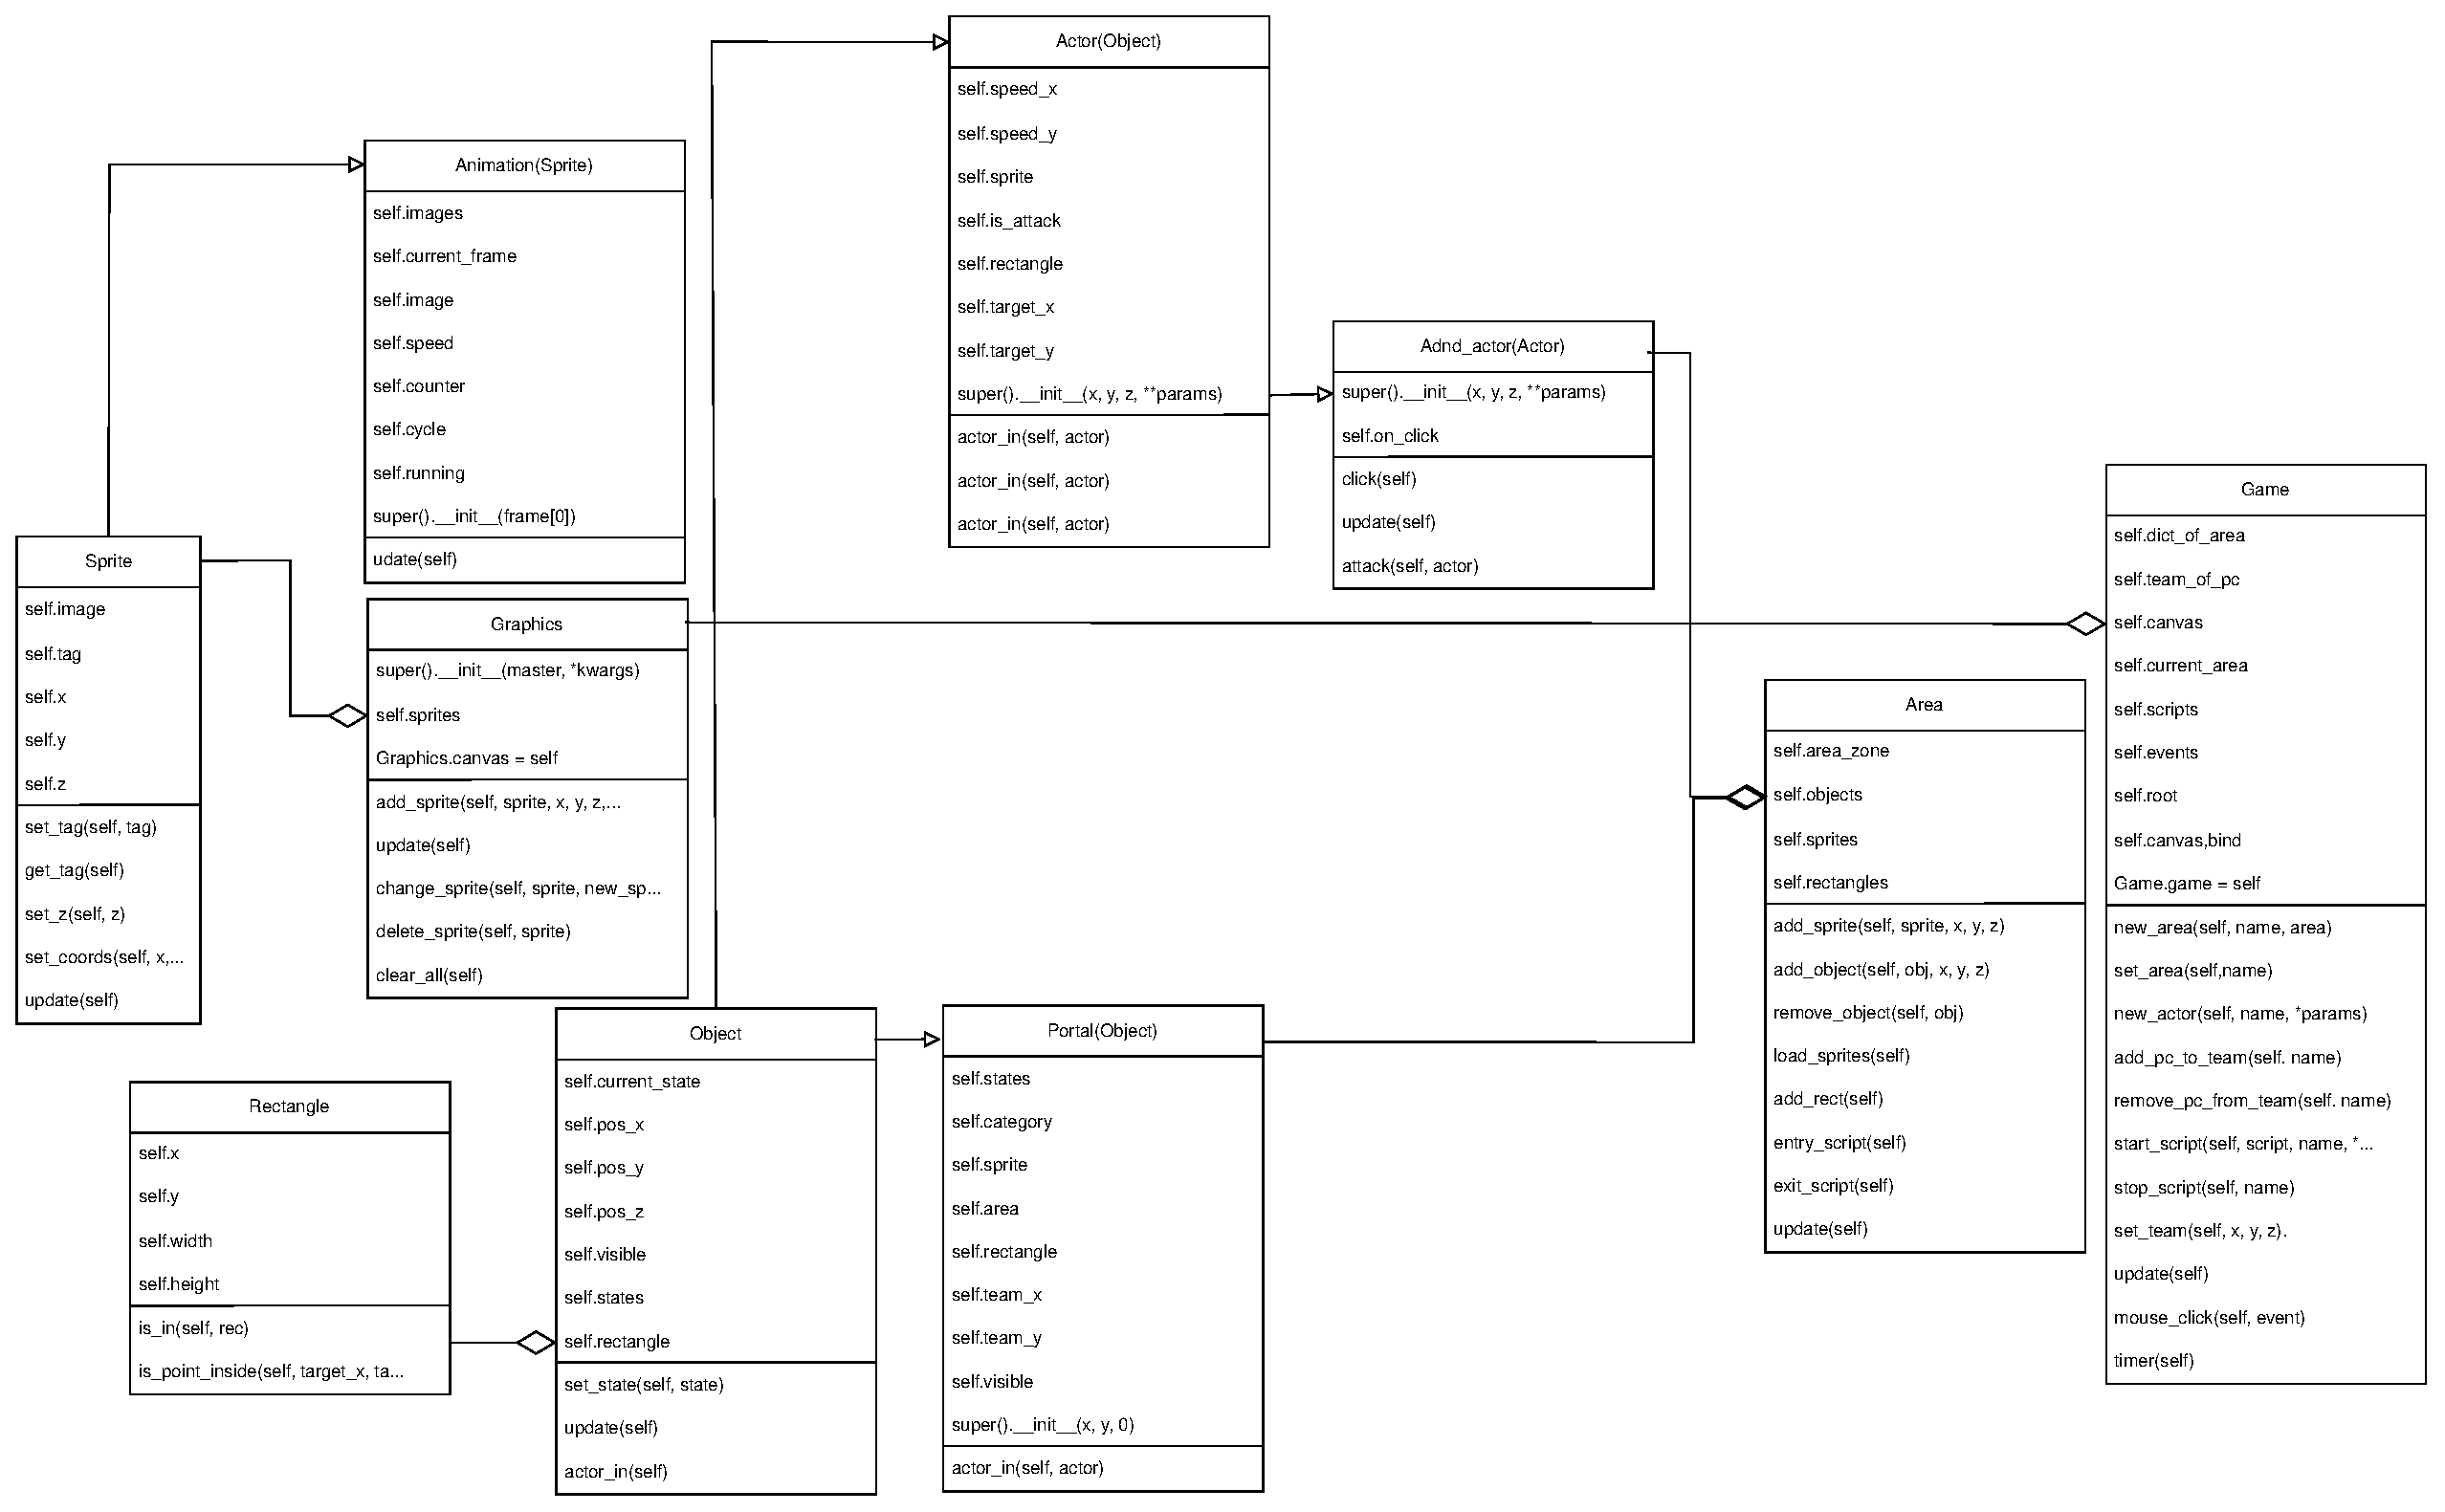
\includegraphics[width=1\linewidth]{diagram}}
	\caption{Диаграмма компонентов}
	\label{diagram:image}
\end{figure}
\paragraph{Описание классов}
\begin{enumerate}
	\item[Graphics] - класс, управляющий спрайтами. Содержит в себе:
	\begin{itemize}
		\item self.sprites - список спрайтов;
		\item add\_sprite(self, sprite x, y, z, image) - добавляет в список спрайт, сохраняет координаты;
		\item change\_sprite(self, sprite new\_sprite) - меняет местами спрайты в списке.
		\item delete\_sprite(self, sprite) - удаляет спрайт из списка.
		\item clear\_all(self) - очищает список спрайтов.
		\item update(self) - добавляет все спрайты из списка на форму.
	\end{itemize}
	\item[Sprite] - класс, хранящий в себе изображение игровых объектов image.
	\begin{itemize}
		\item self.x - координата x.
		\item self.y - координата y.
		\item self.z - координата z.
		\item self.tag - уникальный номер спрайта.
		\item self.image - изображение.
		\item set\_tag(self, tag) - устанавливает tag спрайту.
		\item get\_tag(self) - возвращает tag спрайта.
		\item set\_z(self, z) - устанавливает z координату.
		\item set\_coords(self, new\_x, new\_y) - устанавливает новые координаты.
		\item update(self) - ничего не делает.
	\end{itemize}
	\item[Animation] - класс, хранящий в себе список изображений игровых объектов image. Потомок класса Sprite.
	\begin{itemize}
		\item self.current\_frame - текущий кадр.
		\item self.images  - Загрузка всех кадров анимации.
		\item self.image - Установка начального изображения.
		\item self.speed - скорость анимации.
		\item self.counter - счётчик кадров.
		\item self.cycle - проверка на то что должна ли быть анимация циклично или нет.
		\item self.running - проверка проигрывается ли сейчас анимация.
		\item update(self) - обновляет кадр в анимации.
	\end{itemize}
	\item[Rectangle] - абстрактный класс прямоугольника.
	\begin{itemize}
		\item self.pos\_x - координата x.
		\item self.pos\_y - координата y.
		\item self.width - ширина.
		\item self.height - высота.
		\item is\_in(self, rect) - функция проверки нахождения одного прямоугольника в другом.
		\item is\_point\_inside(self, target\_x, target\_y) - функция проверки точки в пределах прямоугольника.
	\end{itemize}
	\item[Object] - класс, от которого наследуются классы Adnd\_Actor, Actor, Portal.
	\begin{itemize}
		\item self.pos\_x - координата x.
		\item self.pos\_y - координата y.
		\item self.pos\_z - координата z.
		\item self.current\_state - текущее состояние.
		\item self.visible - видимость портала.
		\item self.on\_click - функция клика по объекту.
		\item self.rectangle - прямоугольник объекта.
		\item set\_state(self, state\_name) -устанавливает состояние.
		\item actor\_in(self, actor) - ничего не делает.
		\item update(self) - ничего не делает.
	\end{itemize}
	\item[Portal] - класс объекта для перехода между зонами. Потомок класса Object.
	\begin{itemize}
		\item self.states - состояние портала.
		\item self.sprite - спрайт портала.
		\item self.category - категория.
		\item self.rectangle = - прямоугольник портала.
		\item self.area - зона в которую ведёт портал.
		\item self.team\_x - координата x в  которую нужно разместить команду.
		\item self.team\_y - координата y в  которую нужно разместить команду.
		\item self.visible - видимость портала.
		\item actor\_in(actor) - события, которые произойдут, когда персонаж окажется внутри прямоугольника портала.
	\end{itemize}
	\item[Actor] - класс персонажа, содержащий внутри себя основные поля и методы для перемещения по рабочему окну.
	\begin{itemize}
		\item self.sprite - спрайт персонажа.
		\item self.speed\_x - значение скорости x.
		\item self.speed\_y - значение скорости y.
		\item self.target\_x - координата x в которую должен прийти персонаж.
		\item self.target\_y - координата y в которую должен прийти персонаж.
		\item self.rectangle - прямоугольник персонажа.
		\item self.is\_attack - атакует ли сейчас персонаж.
		\item update(self) - функция обновления координат и состояния персонажа.
		\item search\_position(self, new\_x, new\_y) - поиск координат в которые нужно двигаться персонажу.
		\item stop\_move(self) - остановка движения персонажа.
	\end{itemize}
	\item[Adnd\_Actor] - класс персонажа, содержащий методы связанные с взаимодействием с другими персонажами. Является наследником Actor.
	\begin{itemize}
		\item self.on\_click событие при клике на персонажа
		\item update(self) - функция обновления координат и состояния персонажа.
		\item click(self) - функция вызывается при клике по персонажу.
		\item attack(self, actor) -  функция атаки персонажа по другому персонажу.
	\end{itemize}
	\item[Area] - зона, в которой находятся персонажи и объекты. Содержит следующие поля и методы:
	\begin{itemize}
		\item self.area\_zone - параметр определяющий особенности конкретной зоны.
		\item self.objects - список, хранящий в себе множество объектов.
		\item self.sprites - список фоновых спрайтов.
		\item self.rectangles - прямоугольник зоны.
		\item add\_sprite(self, sprite, x, y, z) - функция добавляет спрайт в зону.
		\item add\_object(self, obj, x, y, z) - функция добавляет объект в зону.
		\item remove\_object(self, obj) - функция удаляет объект из зоны.
		\item load\_sprites(self) - функция загружает все спрайты зоны.
		\item add\_rect(self, rec) - функция добавляет прямоугольник в зону.
		\item entry\_script(self) - функция запускается, когда команда входит в зону.
		\item exit\_script(self) - функция запускается, когда команда выходит из зоны.
		\item update(self) - функция изменяет и проверяет изменение всех объектов в зоне.
	\end{itemize}
	\item[Game] - абстрактный класс, управляющий игрой. Имеет следующие поля и методы:
	\begin{itemize}
		\item self.rpg\_dict\_of\_area - словарь, хранящий в себе множество экземпляров класса Area.
		\item self.team\_of\_pc - список, хранящий в себе имена экземпляров класса Actor с параметром category = "pc".
		\item self.canvas - графика.
		\item self.root - окно для графики.
		\item self.current\_area - параметр хранящий, текущую зону.
		\item self.scripts - словарь для хранения запущенных сценариев.
		\item self.events - словарь для хранения запущенных event`ов сценариев.
		\item self.canvas.bind("<Button-1>", self.mouse\_left.\_click) - обработка клика мыши по рабочему окну.
		\item new\_area(self, name, area) - функция добавляет новую зону в список.
		\item set\_area(self, name) - функция устанавливает текущую зону, загружает графику зоны.
		\item new\_actor(self, name, **params) - функция создаёт класс, потомок от Actor и создаёт поле из параметров, и установление их в начальные значения.
		\item add\_pc\_to\_team(self, pc) - функция добавляет персонажа в команду.
		\item remove\_pc\_from\_team(self, pc) - функция удаляет персонажа из команды.
		\item start\_script(self, script\_function, script\_name, *args) - функция запускает сценарий в отдельном потоке с возможностью остановки и передачи аргументов.
		\item stop\_script(self, script\_name) - функция останавливает сценарий по имени.
		\item set\_team(self, x, y, z) - функция устанавливает координаты персонажей команды.
		\item update(self) - функция вызывается в таймере для обновления всех переменных в текущей зоне.
		\item mouse\_left\_click(self, event) - функция обрабатывает клик мыши.
		\item timer(self) - функция должна вызывать метод update постоянно.
	\end{itemize}
\end{enumerate}

\subsubsection{Реализация графической подсистемы}
Графическая подсистема основана на библиотеке tkinter, которая используется для создания графического интерфейса пользователя. В контексте платформы, tkinter используется для отображения и управления спрайтами — графическими объектами, которые представляют персонажей, предметы и другие элементы игры.
\paragraph{Система спрайтов}
Она реализована через класс Graphics, который расширяет tk.Canvas. Этот класс управляет отображением спрайтов на холсте, их сортировкой по z-координате (что позволяет создать эффект глубины), а также обновлением их позиций. Спрайты могут быть добавлены, перемещены и удалены с холста. Вот пример метода, который добавляет спрайт на холст:
Пример на рисунке \ref{ttk:image}:
\begin{figure}[H]
	\begin{lstlisting}[language=Python]
		def add\_sprite(self, sprite, x, y, z, **kwargs):
			tag = self.create\_image(x, y, image=sprite.image, anchor='center', **kwargs)
			sprite.set\_tag(tag)
			sprite.set\_z(z)
			self.sprites.append(sprite)
			self.sprites.sort(key=lambda sprite: sprite.z)
\end{lstlisting}  
\caption{sprite}
\label{ttk:image}
\end{figure}
\subsubsection{Реализация зон}
Зоны в программе представляют собой различные игровые области. Каждая зона реализована через класс Area, который содержит спрайты и объекты, принадлежащие этой зоне. Класс Area является ключевым элементом в структуре игры, так как он определяет отдельные игровые зоны, которые игрок может исследовать. Каждая зона представляет собой уникальный участок игрового мира со своим набором характеристик и поведения.

Спрайты и объекты: В основе каждой зоны лежат спрайты и объекты. Спрайты — это графические элементы, такие как персонажи, враги или декорации, которые игрок видит на экране. Объекты могут быть как видимыми, так и невидимыми элементами, которые взаимодействуют с игроком или окружением, например, триггеры событий или коллекционные предметы.
Скрипты входа и выхода: entry\_script и exit\_script — это скрипты, которые активируются при входе игрока в зону и при выходе из неё соответственно. Эти скрипты могут использоваться для запуска кат-сцен, начала битв, обновления заданий или любых других событий, которые должны произойти при изменении зоны.
Метод update: Метод update вызывается каждый игровой цикл и отвечает за обновление состояния всех спрайтов и объектов в зоне. Это может включать анимацию спрайтов, проверку столкновений, выполнение игровой логики и многое другое. Если в зоне заданы скрипты входа или выхода, метод update также будет их вызывать в соответствующий момент.
В целом, класс Area обеспечивает структурированное и модульное построение игрового мира, позволяя разработчикам создавать сложные и интерактивные зоны, которые делают игровой процесс более разнообразным и захватывающим. Это также упрощает управление ресурсами и оптимизацию, так как каждая зона может быть загружена и выгружена независимо от остальных.
\subsubsection{Реализация объектов и персонажей}
Объекты и персонажи являются ключевыми элементами игрового мира. Они реализованы через классы Object и Adnd\_Actor соответственно. Object может представлять любой игровой объект, который может взаимодействовать с игроком или окружением. Adnd\_Actor расширяет Object и добавляет дополнительные свойства и методы, специфичные для персонажей, такие как движение, атака и взаимодействие с другими персонажами.
Класс Object служит основой для всех элементов в игре, которые могут взаимодействовать с игроком или средой. Это могут быть предметы, такие как ключи, оружие, сундуки с сокровищами, или даже более абстрактные понятия, такие как ловушки или интерактивные точки.
Класс Adnd\_Actor расширяет Object, добавляя свойства и методы, которые специфичны для персонажей игры. Это включает в себя движение, атаку, взаимодействие с другими персонажами и возможность реагировать на изменения в игровой среде.
Эти классы позволяют разработчикам игр создавать разнообразные и динамичные объекты и персонажи, каждый из которых обладает уникальными характеристиками и способностями. Объекты могут быть простыми и служить одной цели, например, быть предметом для сбора, или же могут быть сложными, выполняя ряд функций в игре. Персонажи, с другой стороны, являются более сложными сущностями, которые могут взаимодействовать с игроком и другими элементами игрового мира на более глубоком уровне, выполняя различные действия, такие как бой, торговля или выполнение заданий.
\subsubsection{Реализация сценариев}
Сценарии в игре используются для создания интерактивных и динамических событий. Они могут быть реализованы как функции, которые запускаются в отдельных потоках, позволяя игре продолжать обрабатывать другие задачи в фоновом режиме. Класс Game содержит методы start\_script и stop\_script для управления этими сценариями. Thread – это отдельный поток выполнения. Это означает, что в вашей программе могут работать две и более подпрограммы одновременно. Но разные потоки на самом деле не работают одновременно: это просто кажется.
Соблазнительно думать, что в программе работают два (или более) разных процессора, каждый из которых выполняет независимую задачу одновременно. Это почти правильно, но это то, что обеспечивает многопроцессорность (multiprocessing).
Запуск потоков (threading) похожа на эту идею, но ваши программы работает только на одном процессоре. Различные задачи, внутри потоков выполняются на одном ядре, а операционная система управляет, когда ваша программа работает с каким потоком.
Поскольку потоки выполняется на одном процессоре, они хорошо подходят для ускорения некоторых задач, но не для всех. Задачи, которые требуют значительных вычислений ЦП и тратят мало времени на ожидание внешних событий, очевидно используя многопоточность не будут выполняться быстрее, вместо этого следует использовать многопроцессорность (multiprocessing).

Архитектура вашей программы при использования многопоточности также может помочь в достижении более чистой архитектуры проекта. Большинство примеров, которые мы рассмотрим в этой статье, не обязательно будут работать быстрее используя потоки. Но использование потоков поможет сделать их архитектуру чище и понятнее. Потоки (Thread)
Теперь, когда у вас есть представление о том, что такое поток, давайте узнаем, как его использовать. Стандартная библиотека Python предоставляет библиотеку threading, которая содержит необходимые классы для работы с потоками. Основной класс в этой библиотеки Thread. Чтобы запустить отдельный поток, нужно создать экземпляр потока Thread и затем запустить его с помощью метода .start() \ref{treading:image}:
\begin{figure}[H]
	\begin{lstlisting}[language=Python]
		import threading
		import time
		def thread_function(name):
			logging.info("Thread %s: starting", name)
			time.sleep(2)
			logging.info("Thread %s: finishing", name)
		if __name__ == "__main__":
			format = "%(asctime)s: %(message)s"
			logging.basicConfig(format=format, level=logging.INFO,
			datefmt="%H:%M:%S")
			logging.info("Main    : before creating thread")
			x = threading.Thread(target=thread_function, args=(1,))
			logging.info("Main    : before running thread")
			x.start()
			logging.info("Main    : wait for the thread to finish")
			# x.join()
			logging.info("Main    : all done")
		x = threading.Thread(target=thread_function, args=(1,))
		x.start()
	\end{lstlisting}  
	\caption{tread.start}
	\label{treading:image}
\end{figure}
Когда создается поток Thread, вы передаете ему функцию и список, содержащий аргументы этой функции. В нашем примере мы говорим Thread, чтобы он запустил функцию thread\_function() и передаем ему 1 в качестве аргумента.

Сама по себе функция thread\_function() мало что делает. Она просто выводит некоторые сообщения с промежутком time.sleep() между ними.
Демоны потоков
В информатике daemon (демон) – это процесс, который работает в фоновом режиме.

Python потоки имеет особое значение для демонов. Демон потока (или как еще его можно назвать демонический поток) будет остановлен сразу после выхода из программы. Один из способов думать об этих определениях – считать демон потока как потоком, который работает в фоновом режиме, не беспокоясь о его завершении.

Если в программе запущены потоки, которые не являются демонами, то программа будет ожидать завершения этих потоков, прежде чем сможет завершится. Тем не менее, потоки, которые являются демонами, при закрытие программы просто убиваются, в каком бы они состояние ни находились.
join()
Демонические потоки удобны, но что делать, если вы хотите дождаться остановки потока? Чтобы указать одному потоку дождаться завершения другого потока, вам нужно вызывать .join().  Если вызвать .join(), этот оператор будет ждать, пока не завершится любой вид потока.
\subsubsection{Вычисление пересечения прямоугольников}
Для определения столкновений и взаимодействий между объектами используется класс Rectangle. Он содержит методы, такие как is\_in, который проверяет, находится ли один прямоугольник внутри другого, и is\_point\_inside, который проверяет, находится ли точка внутри прямоугольника. Вот пример метода is\_point\_inside на рисунке \ref{tttk:image}:
\begin{figure}[H]
	\begin{lstlisting}[language=Python]
		def is\_point\_inside(self, target\_x, target\_y):
		return (self.x <= target\_x <= self.x + self.width) and
		(self.y <= target\_y <= self.y + self.height)
		Этот метод использует логические операторы для проверки, находится ли точка (target\_x, target\_y) в пределах прямоугольника, определенного координатами (x, y) и размерами (width, height).
\end{lstlisting}  
\caption{rectangle}
\label{tttk:image}
\end{figure}

